\begin{abstract}
	In tale esperienza si è proceduto ad effettuare una misura della costante  Boltzmann.
	Per effettuare tali misure si è proceduto a misurare il rumore termico prodotto da
	alcune resistenze di prova, di vari valori.
	Dai dati ottenuti si è ottenuto $k_{sper}=$\SI{e-21}{ }
	a fronte di un $k_{att}=$\SI{e-21}{ }.
\end{abstract}
\section{Note preliminari e setup}
	Essendo l'apparato impiegato sensibile ad eventuali rumori si è proceduto a realizzare i collegamenti più corti e schiacciati possibile per minimizzare gli effetti di induzione;
	effettuando un montaggio a blocchi e verificando singolarmente il funzionamento circuitali
	delle vari circuiti che costituiscono l'apparato di misura impiegato.

	Si è proceduto inoltre  ad alimentare le componentistiche impiegando le medesime linee
	di distribuzione, tensioni $V_{+}=$ \SI{5.00(4)}{\volt} e $V_{-}=$ \SI{-5.01(4)}{\volt}.
	Per ridurre ulteriormente il rumore introdotto dalle tensioni di alimentazione
	si è proceduto a montare il circuito in \figurename{ \ref{fig:prel}}.
	\begin{figure}[h]
		\begin{minipage}{0.5\textwidth}
			\centering
			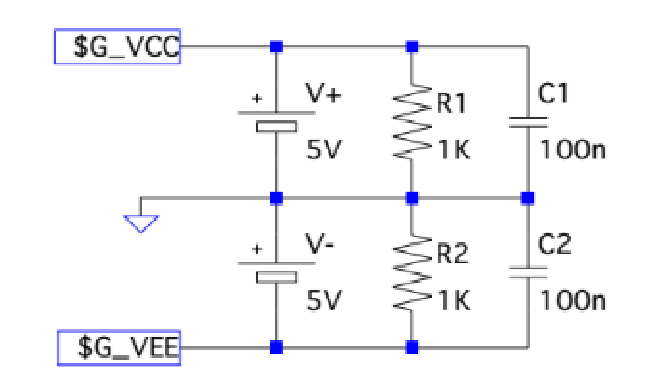
\includegraphics{prelim.png}
			\caption{Circuito di filtro alimentazioni.}
			\label{fig:prel}
		\end{minipage}
		\begin{minipage}{0.3\textwidth}
			\begin{tabular}{l@{ }c@{ }l}
				$R_{1}$& = &\SI{9.84(9)}{\kilo\ohm}\\
				$R_{2}$& = &\SI{9.74(9)}{\kilo\ohm}\\
				$C_1$& = &\SI{113(5)}{\nano\farad}\\
				$C_2$& = &\SI{106(5)}{\nano\farad}\\
			\end{tabular}
		\end{minipage}
	\end{figure}
\section{Strumentazione}
	Per questa esperienza sono state impiegate le seguenti strumentazioni, in aggiunta a quelle
	usualmente in dotazione sul banco di lavoro.
	\begin{itemize}
		\item 1 INA114: Precision instrumentation amplifier
		\item 2 IC AD708: ultra low offset dual op-amp
		\item 1 AD736: true rms-to-dc converter
		\item un set di resistori e capacitori coi reofori tagliati; impiegati nelle realizzazioni circuitali.
	\end{itemize}
\section{Metodo di misura}
	Per effettuare le misure è stato realizzato l'apparato in \figurename{ \ref{fig:completo}}
	verificando per ciascuno dei blocchi in figura l'operatività.
	Effettuate tali verifiche sono stati collegati tra loro i vari blocchi
	e sono stati acquisiti i valori di tensione, $V_{RMS}$, letti in continua sul voltmetro,
	per vari valori di resistenze in dotazione.

	Dalla campionatura ottenuta attraverso un fit a tre parametri sono state ottenuti i valori
	di $V_{0n}$, $R_{T}$, $R_{n}$; rispettivamente : il rumore in uscita a resistenza nulla; la resistenza equivalente del rumore serie dell'amplificatore riferito all'ingresso ed il rapporto tra il rumore parallelo; il rumore serie dell’amplificatore, riferiti all’ingresso.

	\begin{figure}[h]
			\centering
			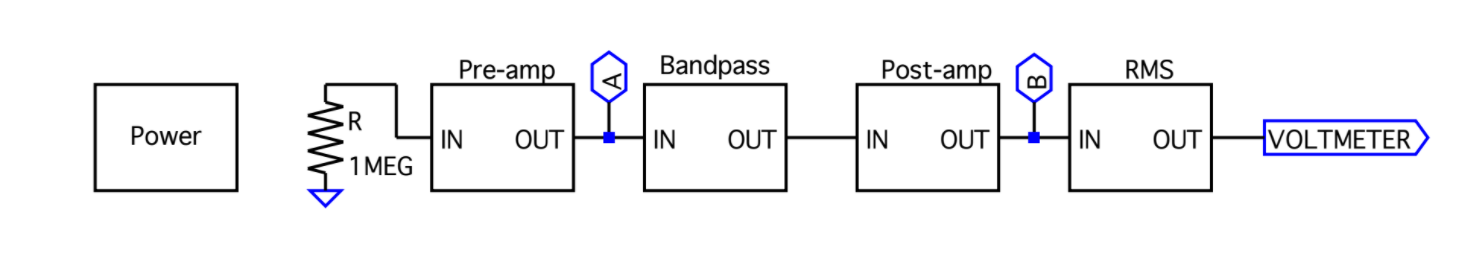
\includegraphics[scale = 0.4]{completo.png}
			\caption{schema dell'apparato di misura.}
			\label{fig:completo}
	\end{figure}

	Tali valori, essendo determinati da $k_{B}$ da relazioni descritte nel seguito, hanno permesso
	di ricavare una misura della costante di Boltzmann.
